\newpage
\subsection{Caso d'uso UC7 - Interazione Con Proprio Profilo Utente}
\label{UC7}
\begin{figure}[ht]
	\centering
	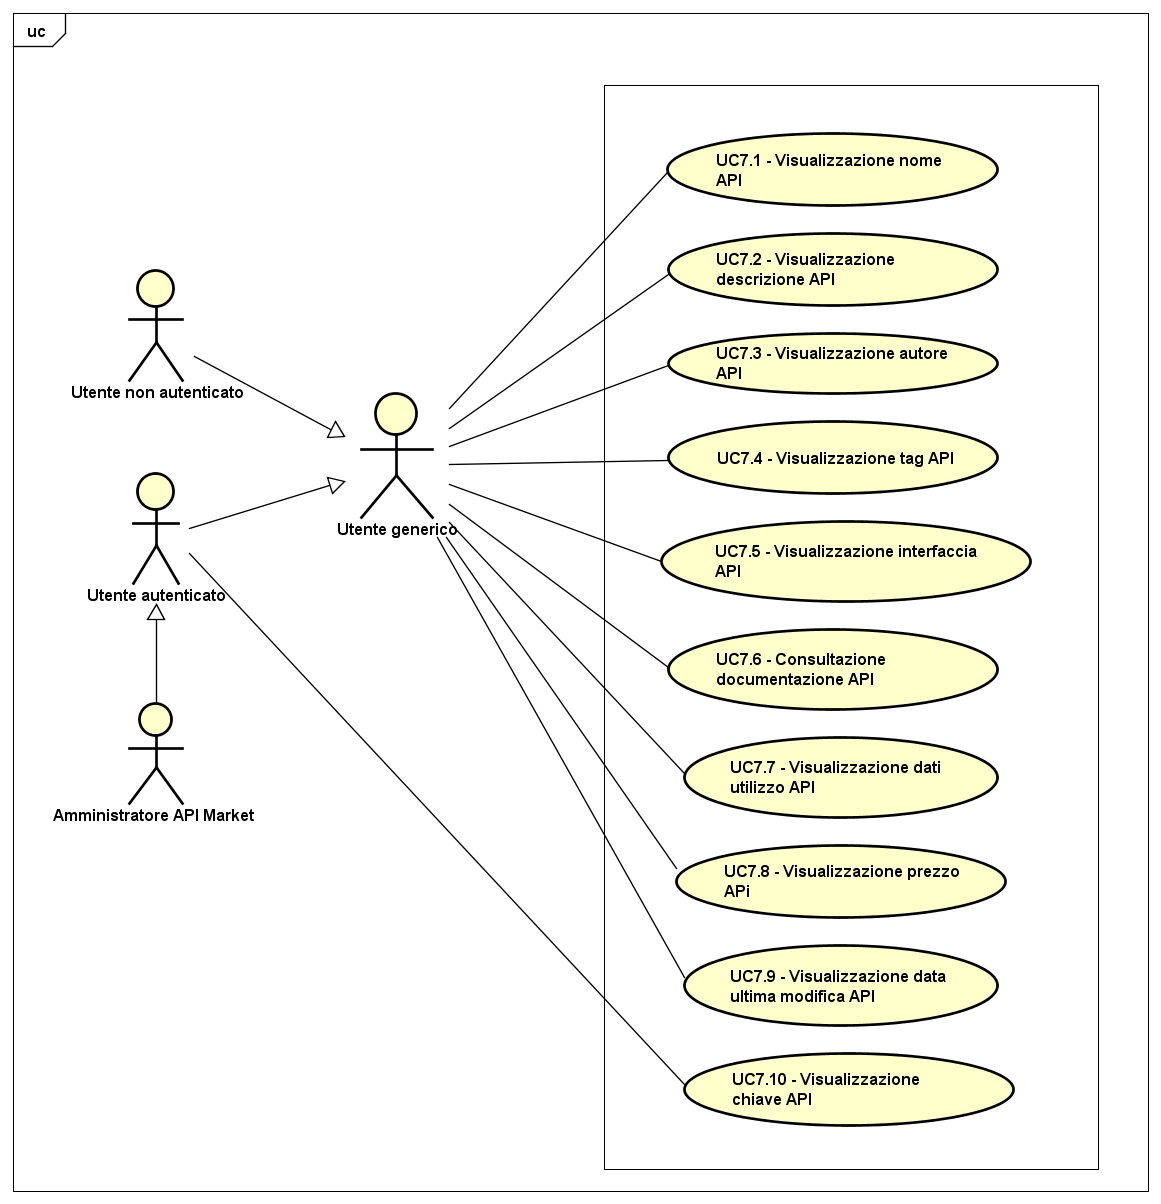
\includegraphics[scale=0.45]{UML/UC7.png}
	\caption{UC7: Interazione Con Proprio Profilo Utente}
\end{figure}

\begin{longtable}{ l | p{11cm}}
	\hline
	\rowcolor{Gray}
	\multicolumn{2}{c}{UC7 - Interazione Con Proprio Profilo Utente}\\
	\hline
	
	 \textbf{Attori} & Utente autenticato  \\
	\textbf{Descrizione} & L'utente puo' interagire con il proprio profilo utente, visualizzare i propri dati e gestirlo in vari modi  \\
	\textbf{Pre-Condizioni} & L'utente e' autenticato in APIMarket\\
	\textbf{Post-Condizioni} & L'utente ha scelto l'interazione con il proprio profilo\\
	\textbf{Scenario Principale} & 
	\begin{enumerate*}[label=(\arabic*.),itemjoin={\newline}]
		\item L'utente puo' gestire il proprio profilo (UC7.1)
		\item L'utente puo' visualizzare il proprio profilo (UC7.2)
	\end{enumerate*}\\
\end{longtable}
